\subsection{Choix des matériaux}
La sélection des matériaux pour ce projet a été effectuée en tenant compte de critères techniques, économiques et pratiques. Chaque composant a été analysé afin de garantir une adéquation entre les propriétés mécaniques requises et les contraintes liées à notre contexte de travail.\\
Pour répondre aux exigences du projet, les matériaux ont été évalués selon plusieurs aspects :

\begin{itemize}
    \item \underline{Propriétés mécaniques :} leurs caractéristiques (module de Young, limite d’élasticité, résistance maximale en traction) devraient permettre de répondre aux sollicitations prévues.
    \item \underline{Contraintes économiques :} le coût des matières premières et de leur usinage a été un facteur déterminant, certains matériaux performants ayant été écartés en raison de leur prix élevé.
    \item \underline{Accessibilité et facilité de fabrication :} une attention particulière a été portée à la disponibilité des matériaux et à leur compatibilité avec les outils disponibles (imprimantes 3D, machines de découpe, etc.).
    \item \underline{Résistance thermique :} les matériaux sélectionnés devraient conserver leurs propriétés dans les plages de température attendues.\\
\end{itemize}

Le tableau suivant présente les propriétés mécaniques, les coûts estimés et les températures maximales d’utilisation des matériaux sélectionnés. Ces données ont guidé nos choix pour chaque composant du projet.

\begin{table}[h!]
    \centering
    \begin{tabular}{|p{2cm}|p{1.2cm}|p{1.8cm}|p{1.8cm}|p{3cm}|p{2cm}|p{0.8cm}|}
        \hline
        Matériau & Densité (kg/m$^3$) & Module de Young (GPa) & Limite d'élasticité (MPa) & Résistance maximale en traction (MPa) & Température max. (°C) & Coût \\ \hline
        Alu 6061-T6 & 2700 & 69 & 276 & 310 & 150 & €€ \\ \hline
        Alu 7075-T6 & 2810 & 71 & 503 & 572 & 150 & €€€ \\ \hline
        Acier (304) & 8000 & 193 & 240 & 620 & 650 & €€€€ \\ \hline
        Laiton & 8530 & 105 & 300 & 450 & 200 & €€ \\ \hline
        GFRP (163,g/m$^2$) & 1850 & 25 & -- & 500 & 150 & €€€ \\ \hline
        PETG & 1280 & 1,81 (x-y) / 1,54 (z) & 50--55 & 55--60 (x-y) / 35--40 (z) & 80--90 & € \\ \hline
        POM-C & 1410 & 2,8--3,2 & 60--70 & 65--75 & 100--110 & €€ \\ \hline
        Nylon 6 & 1140 & 2,5 & 70 & 80 & 120 & €€ \\ \hline
    \end{tabular}
    \caption{Propriétés mécaniques et coût des matériaux sélectionnés}
    \label{tab:choix_materiaux}
\end{table}

Aux vues des données définies dans le \autoref{tab:choix_materiaux}, nous choississons :
\begin{itemize}
    \item Structures porteuses (tubes, trappes, coiffe, cages...) en \textbf{fibre de verre} pour sa résistance en traction et sa légèreté. La fabrication des pièces est faisable sur-mesure avec des moyens très abordables avec des protocoles spécifiques.
    \item Éléments internes structuraux soumis à de larges contraintes (pièces de séparation inter-étage, bague de maintien du parachute...) en aluminium \textbf{6061-T6 ou 7075-T6} -- usinés par un usineur spécialisé en aluminium -- pour sa légèreté, sa résistance et sa disponibilité auprès des usineurs.
    \item Pièces internes soumises à des frottements avec des éléments en aluminium (aérofreins, palier de la vis sans fin...) réalisés en \textbf{POM-C ou en laiton} qui possèdent un coefficient de friction avec l'aluminium très faible sans graisse supplémentaire.
    \item Éléments internes non structuraux réalisés en \textbf{PLA/PETG} pour la simplicité de fabrication via impression 3D.
\end{itemize}

Dans la continuité de notre apprentissage, nous souhaitons remercier le \textbf{FabLab} de l'école pour nous avoir permis de nous former sur une CNC 3 axes afin d'usiner divers pièces en aluminium (bagues parachute, crochets...) et pièces composites (ailerons) et ainsi maîtriser de nouvelles compétences tout en rduisant notre dépendance à des usineurs externes.
\subsubsection{Précision du protocole de fabrication des fuselages porteurs}
\label{subsubsec:fab_tub}

Lors du dimensionnement de nos deux étages, nous avons opté pour des tubes dits en "\textbf{peau porteuse}", c'est-à-dire qui
supporteront chacun l'entièreté des composants dans la fusée sans renforts internes. Les fuselages des deux étages sont
entièrement en \textbf{fibre de verre} (163 g/cm$^2$) pour un ratio rigidité/masse optimal, avec un diamètre interne de 100 mm,
pour l'étage inférieur et 80 mm pour l'étage supérieur. Nous avons opté pour des tubes en aluminium comme mandrins afin de
minimiser au maximum la flèche à vide du tube, et donc la flèche globale après assemblage. L'ensemble des blocs de chaque étage sera donc fixé au tube porteur en fibre de verre.\\

\begin{figure}[h!]
    \centering
    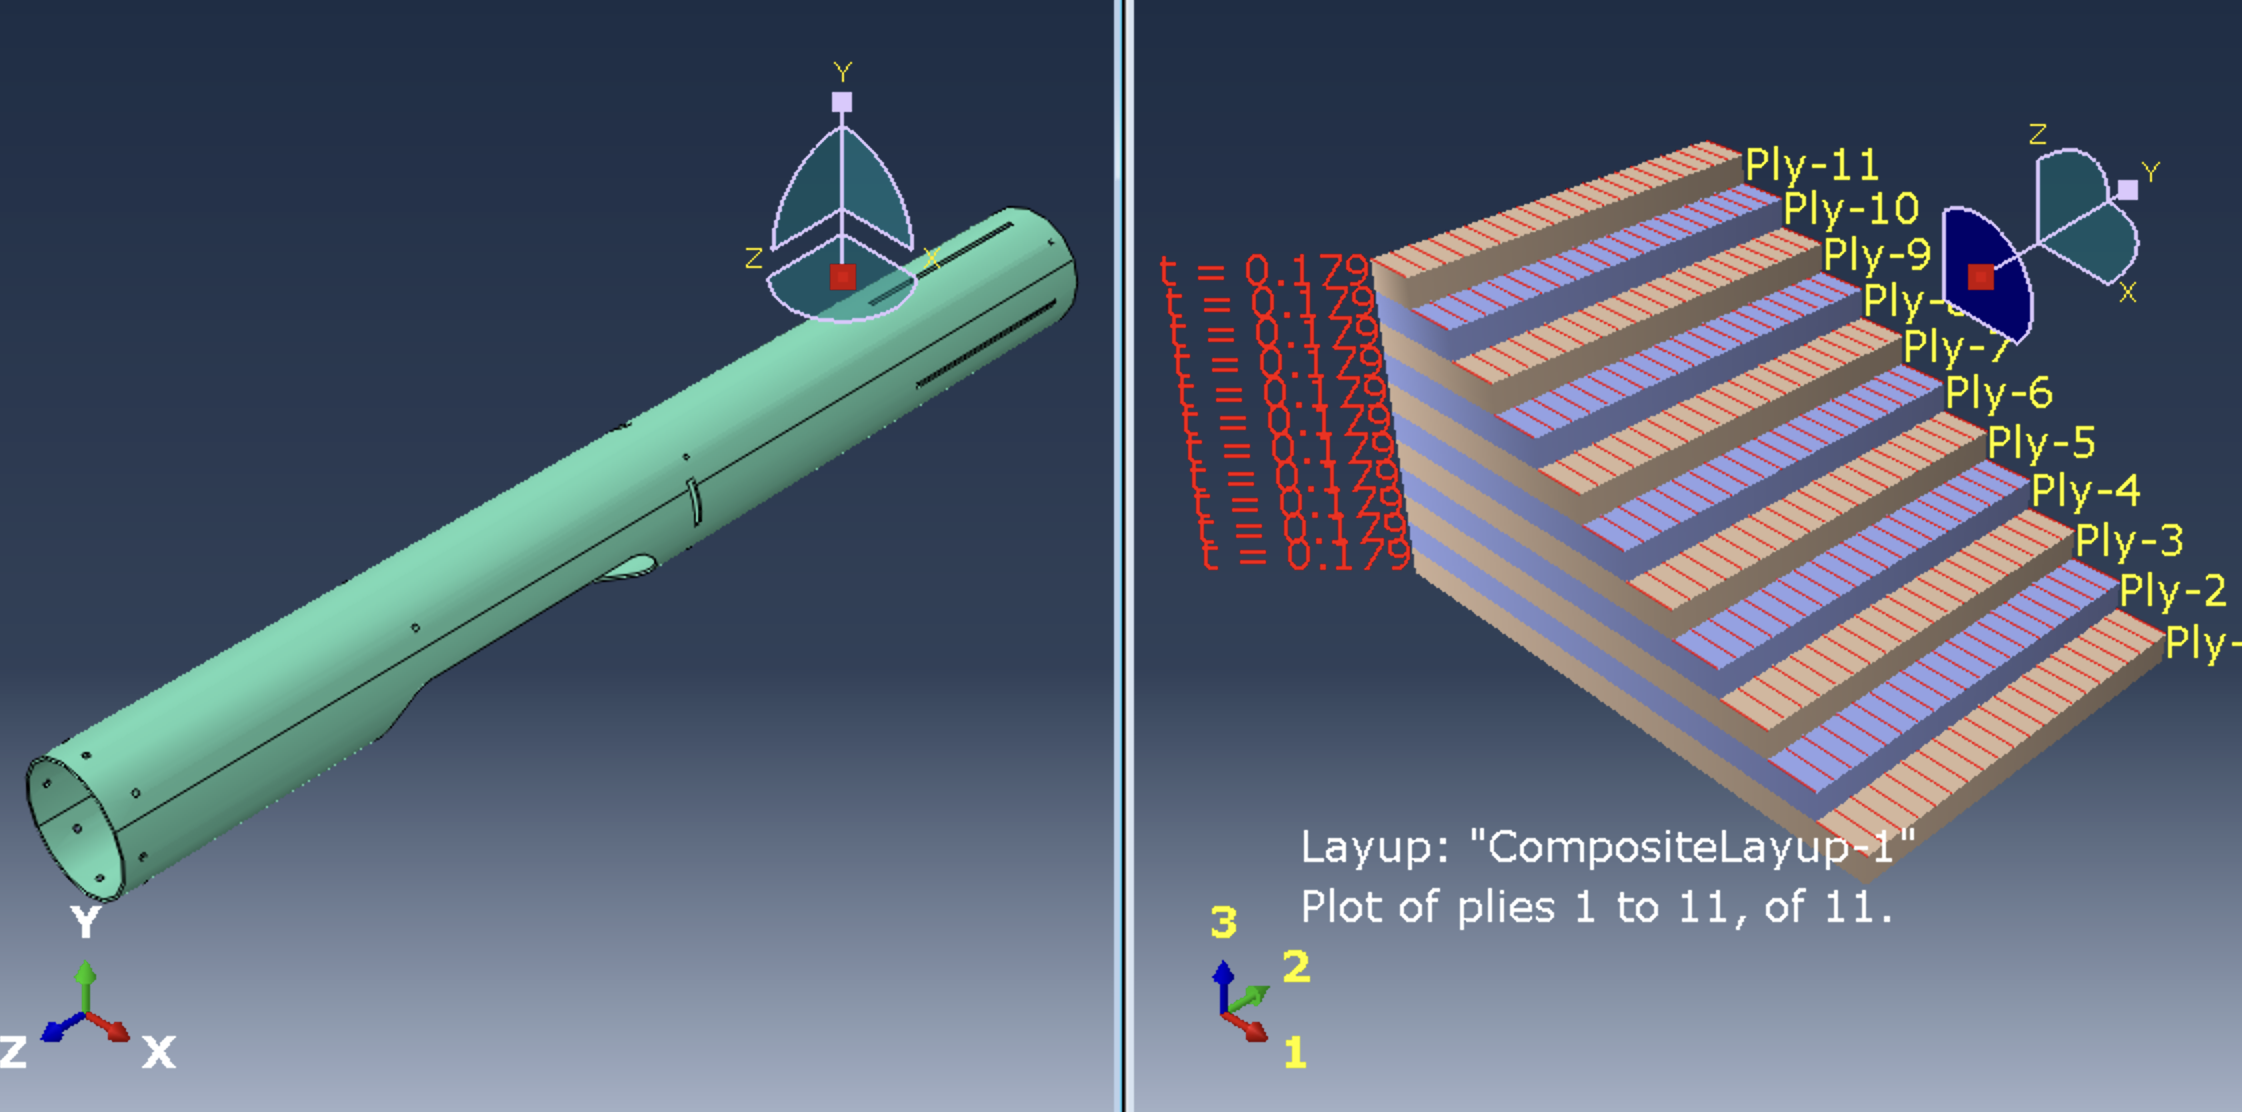
\includegraphics[width=0.6\linewidth]{figures/meca/simu_composite.png}
    \caption{Définition du composite du tube porteur du premier étage}
    \label{fig:stress_loquet}
\end{figure}

L'épaisseur idéale, offrant un compromis entre rigidité et légèreté, se situe entre :
\begin{itemize}
    \item 1,5 mm (rigidité faible),
    \item 2,5 mm (rigidité optimale, mais masse élevée).\\
\end{itemize}


\noindent
\textbf{Étapes de fabrication :}

\begin{enumerate}
    \item \textbf{Préparation de la surface} :
    \begin{itemize}
        \item Ponçage manuel du tube, suivi d'un nettoyage à l'\textit{acétone}.
        \item Application d'un film plastique pour un démoulage instantané du tube sur le mandrin.
    \end{itemize}
    \item \textbf{Fabrication du tube en fibre de verre} :
    \begin{itemize}
        \item Application de la résine sur la fibre, dans le sens des fibres, pour réaliser les 11 couches. Un calcul optimal
        pour permettre d'imprégner en bonne proportion la fibre et atteindre \textbf{291 g/m$^2$} en surface massique du
        composite stratifié final (avec 5\% de marge pour la fabrication de résine).
        \item Vérification de l'état de la résine et port des \acrfull{EPI}.
        \item Pose d'un \textit{film plastique} sur toute la surface du tube pour créer une couche protectrice homogène sur la
        surface extérieure afin de la traiter (ponçage) et d'obtenir la masse et le niveau de surface souhaité.
    \end{itemize}
    \item \textbf{Démoulage du tube} :
    \begin{itemize}
        \item La résine utilisée au cours de la fabrication est une résine epoxy de EasyComposites dont les propriétés mécaniques
        nous permettent d'obtenir nos stratifiés résistants à de nombreux décollages. La période de séchage est de 24 heures à
        température ambiante (18-25°) avant de retirer le film supérieur.
        \item La séparation des deux tubes est facilitée avec le film plastique (démoulage en 0,19s).
    \end{itemize}
\end{enumerate}

\subsubsection{Choix des vis}
Dans le choix des éléments de fixation, nous avons fait le choix d'associer le diamètre de vis à une fonction spécifique. Nous avons défini que l'ensemble des vis M3 sera pour les composants tels cartes électroniques et pièces PLA de maintien ; les vis M4 pour l'ensemble des fixations sur le second étage ; et enfin en M5 sur le sytème de séparation et le premier étage.
Ce choix s'est défini pour ainsi ne mélanger aucune vis et essayer de standardiser les éléments sans difficulté de mesure.

\newpage
\subsubsection{Réalisation mécanique et composite}

\subsubsubsection{Prototypage par impression 3D et validation d’intégration}
Avant toute fabrication métallique, nous avons d’abord imprimé en 3D les pièces modélisées sur \textsc{\acrshort{CATIA}} afin de
valider l’intégration et le bon fonctionnement des parties mécaniques mobiles. Cette étape nous permet de confronter la
\acrshort{CAO} à la réalité : contrôle des encombrements, vérification des interfaces, définition d’un ordre de montage
réaliste, et confirmation des jeux fonctionnels nécessaires pour éviter les points durs.\\

Le mécanisme de séparation illustre cette démarche. Nous avons imprimé et testé plus de six versions différentes avant d’aboutir
à la version finale. À chaque itération, nous avons corrigé des défauts identifiés en essai (rigidité locale insuffisante, zones
de frottement, interférences, tolérances trop serrées) jusqu’à obtenir une solution intégrable, répétable au montage et fiable en
fonctionnement.

\subsubsection{Usinage \acrshort{CNC} des pièces aluminium au Fablab}

Une fois le design figé et validé en impression 3D, nous avons lancé la fabrication des pièces définitives en aluminium. Les
pièces usinées en interne ont été réalisées sur la \acrshort{CNC} de l’école (Mechanika Pro M). Pour les géométries les plus
exigeantes, nous avons fait appel à un industriel équipé d’une \acrshort{CNC} 5 axes. L’objectif est de limiter les reprises,
d’améliorer la précision sur des formes difficiles d’accès en 3 axes et de garantir l’alignement des surfaces fonctionnelles
(perpendicularités, coaxialités, profils).

\subsubsubsection{Préparation \acrshort{CAM} sous Fusion 360}
Pour les pièces usinées par nos soins, nous réalisons la préparation \textit{\acrfull{CAM}} dans \textsc{Fusion 360}. Ce logiciel
d’Autodesk intègre un module de programmation d’usinage permettant de transformer une géométrie issue de la CAO en trajectoires
outils exécutables par une machine-outil à commande numérique.\\

Les pièces conçues sur \textsc{\acrshort{CATIA}} sont importées dans \textsc{Fusion 360} (généralement au format neutre STEP),
puis nous définissons le \textit{setup} d’usinage : description du brut, choix de l’origine pièce (zéro programme), orientation
des axes et positionnement cohérent avec le montage sur la CNC. Nous construisons ensuite une séquence d’opérations logique
(dégrossissage, surfaçage, poches, contournages, perçages, finition). Le choix des outils et des paramètres (avance, vitesse de
rotation, profondeur de passe, stratégie d’engagement) est ajusté selon la matière usinée, la rigidité de la pièce et le bridage,
afin d’obtenir un compromis robuste entre temps d’usinage, qualité géométrique et sécurité machine. Enfin, la simulation intégrée
permet de vérifier l’enlèvement de matière et d’anticiper les collisions potentielles (outil, porte-outil, bridage).

\begin{figure}[htbp]
    \centering
    \begin{minipage}{0.49\linewidth}
        \centering
        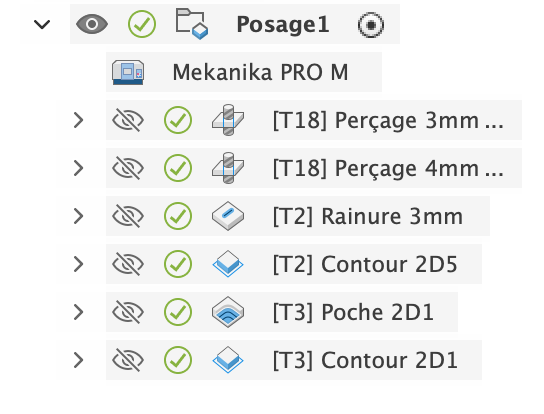
\includegraphics[width=\linewidth]{figures/meca/usion_etapes.png}
        \caption*{Arborescence des opérations d’usinage dans \textsc{Fusion 360}.}
    \end{minipage}\hfill
    \begin{minipage}{0.49\linewidth}
        \centering
        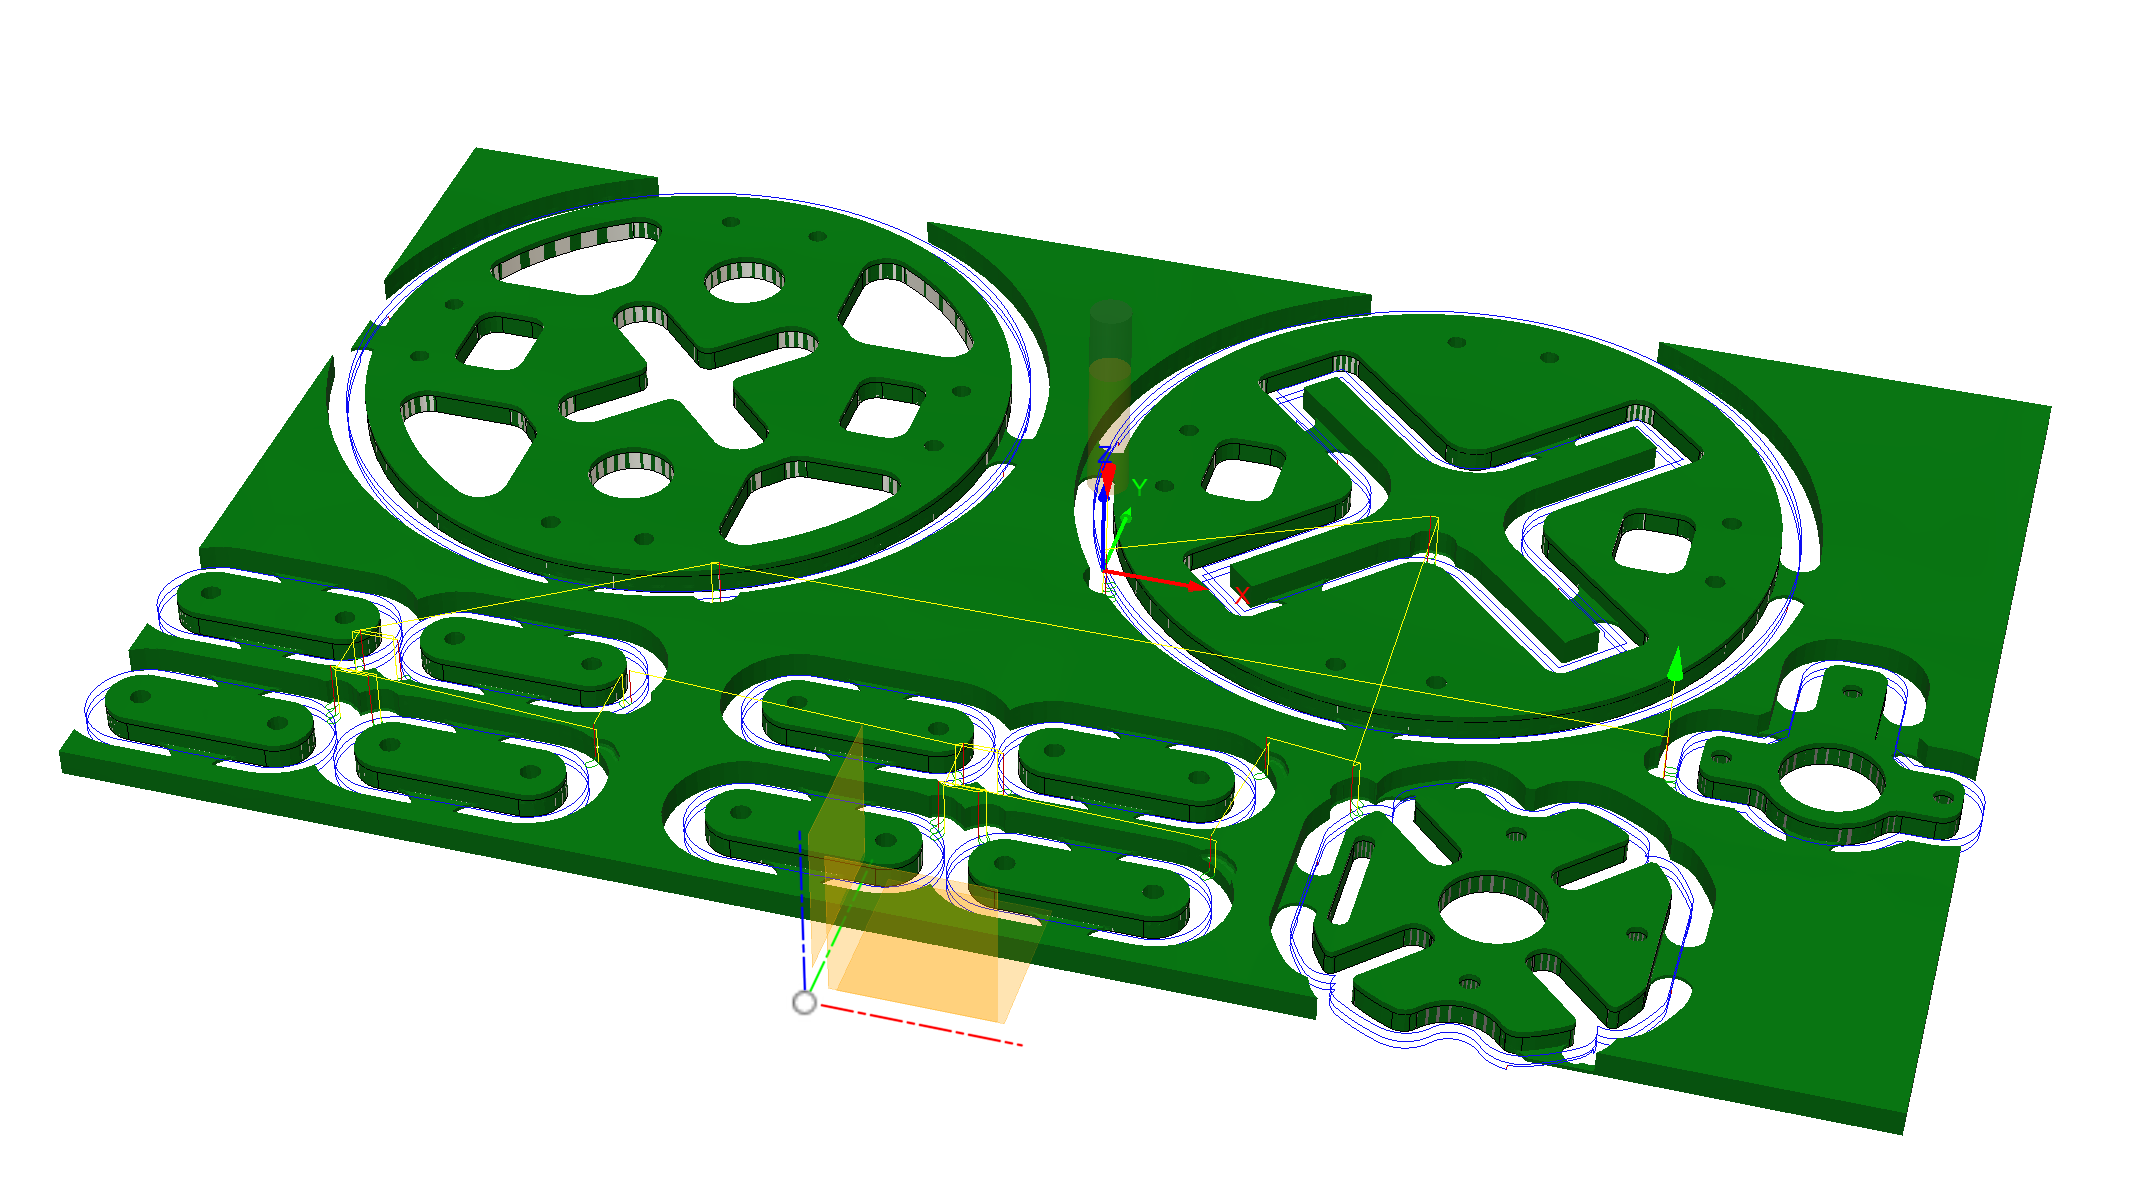
\includegraphics[width=\linewidth]{figures/meca/fusion_previsualisation.png}
        \caption*{Prévisualisation du brut et du résultat après opérations.}
    \end{minipage}
    \caption{Préparation \acrshort{CAM} sous \textsc{Fusion 360} : définition des opérations et validation par simulation.}
    \label{fig:fusion_cam}
\end{figure}

\subsubsubsection{Maintien au brut : rôle des onglets d’usinage}
Lors du détourage final, nous conservons volontairement les pièces attachées au brut par des \textit{onglets}. Sans ces ponts
de matière, la pièce peut se libérer en fin d’usinage, vibrer, se déplacer ou être éjectée, ce qui dégrade la précision et
augmente le risque de casse d’outil. Les onglets garantissent un maintien rigide jusqu’à la dernière passe. Une fois l’usinage
terminé, nous coupons les onglets puis nous reprenons localement la pièce pour supprimer les marques résiduelles.

\begin{figure}[htbp]
    \centering
    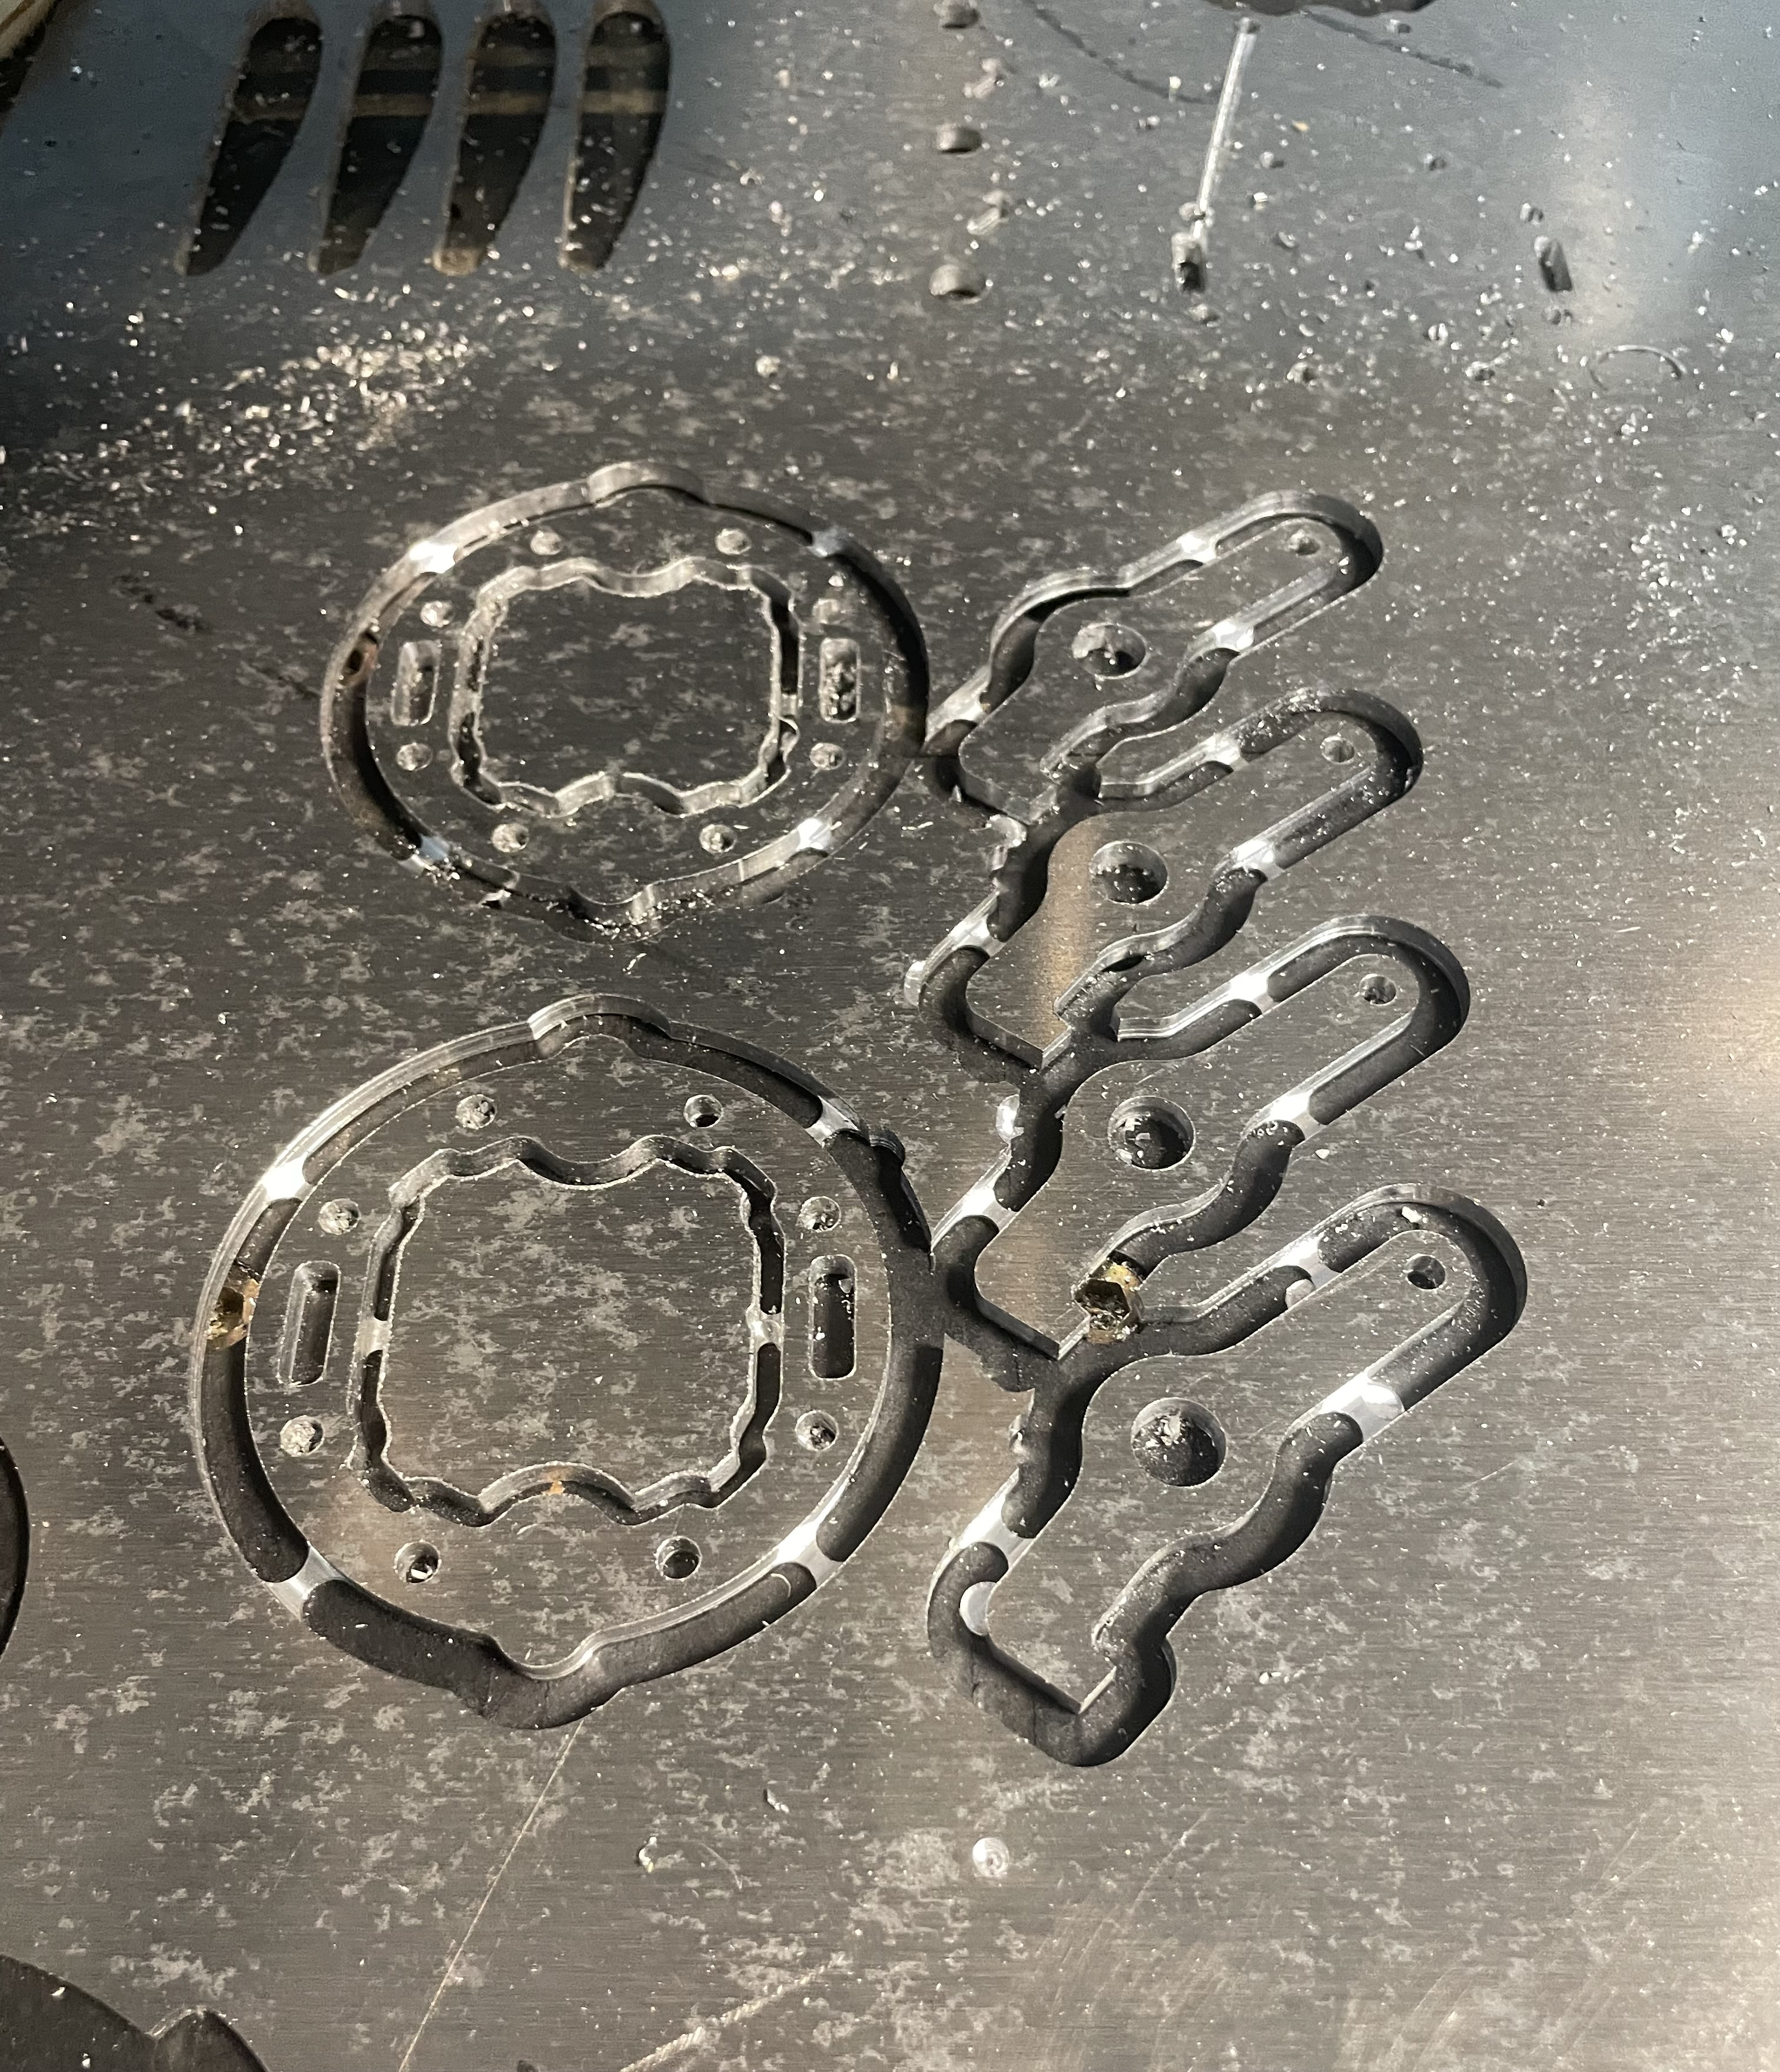
\includegraphics[width=0.5\linewidth]{figures/meca/cnc_onglets_brut.png}
    \caption{Pièce usinée restant solidaire du brut grâce aux onglets de maintien.}
    \label{fig:cnc_onglets}
\end{figure}

\subsubsubsection{Finition des pièces : ébavurage et ponçage}
Après séparation du brut, nous réalisons un ébavurage complet puis un ponçage. L’objectif ne se limite pas à l’aspect visuel :
supprimer les bavures et arêtes vives améliore l’assemblage, limite le risque de grippage sur les zones en friction, et
fiabilise les interfaces mécaniques lorsque plusieurs pièces sont en contact dans un mécanisme.

\begin{figure}[htbp]
    \centering
    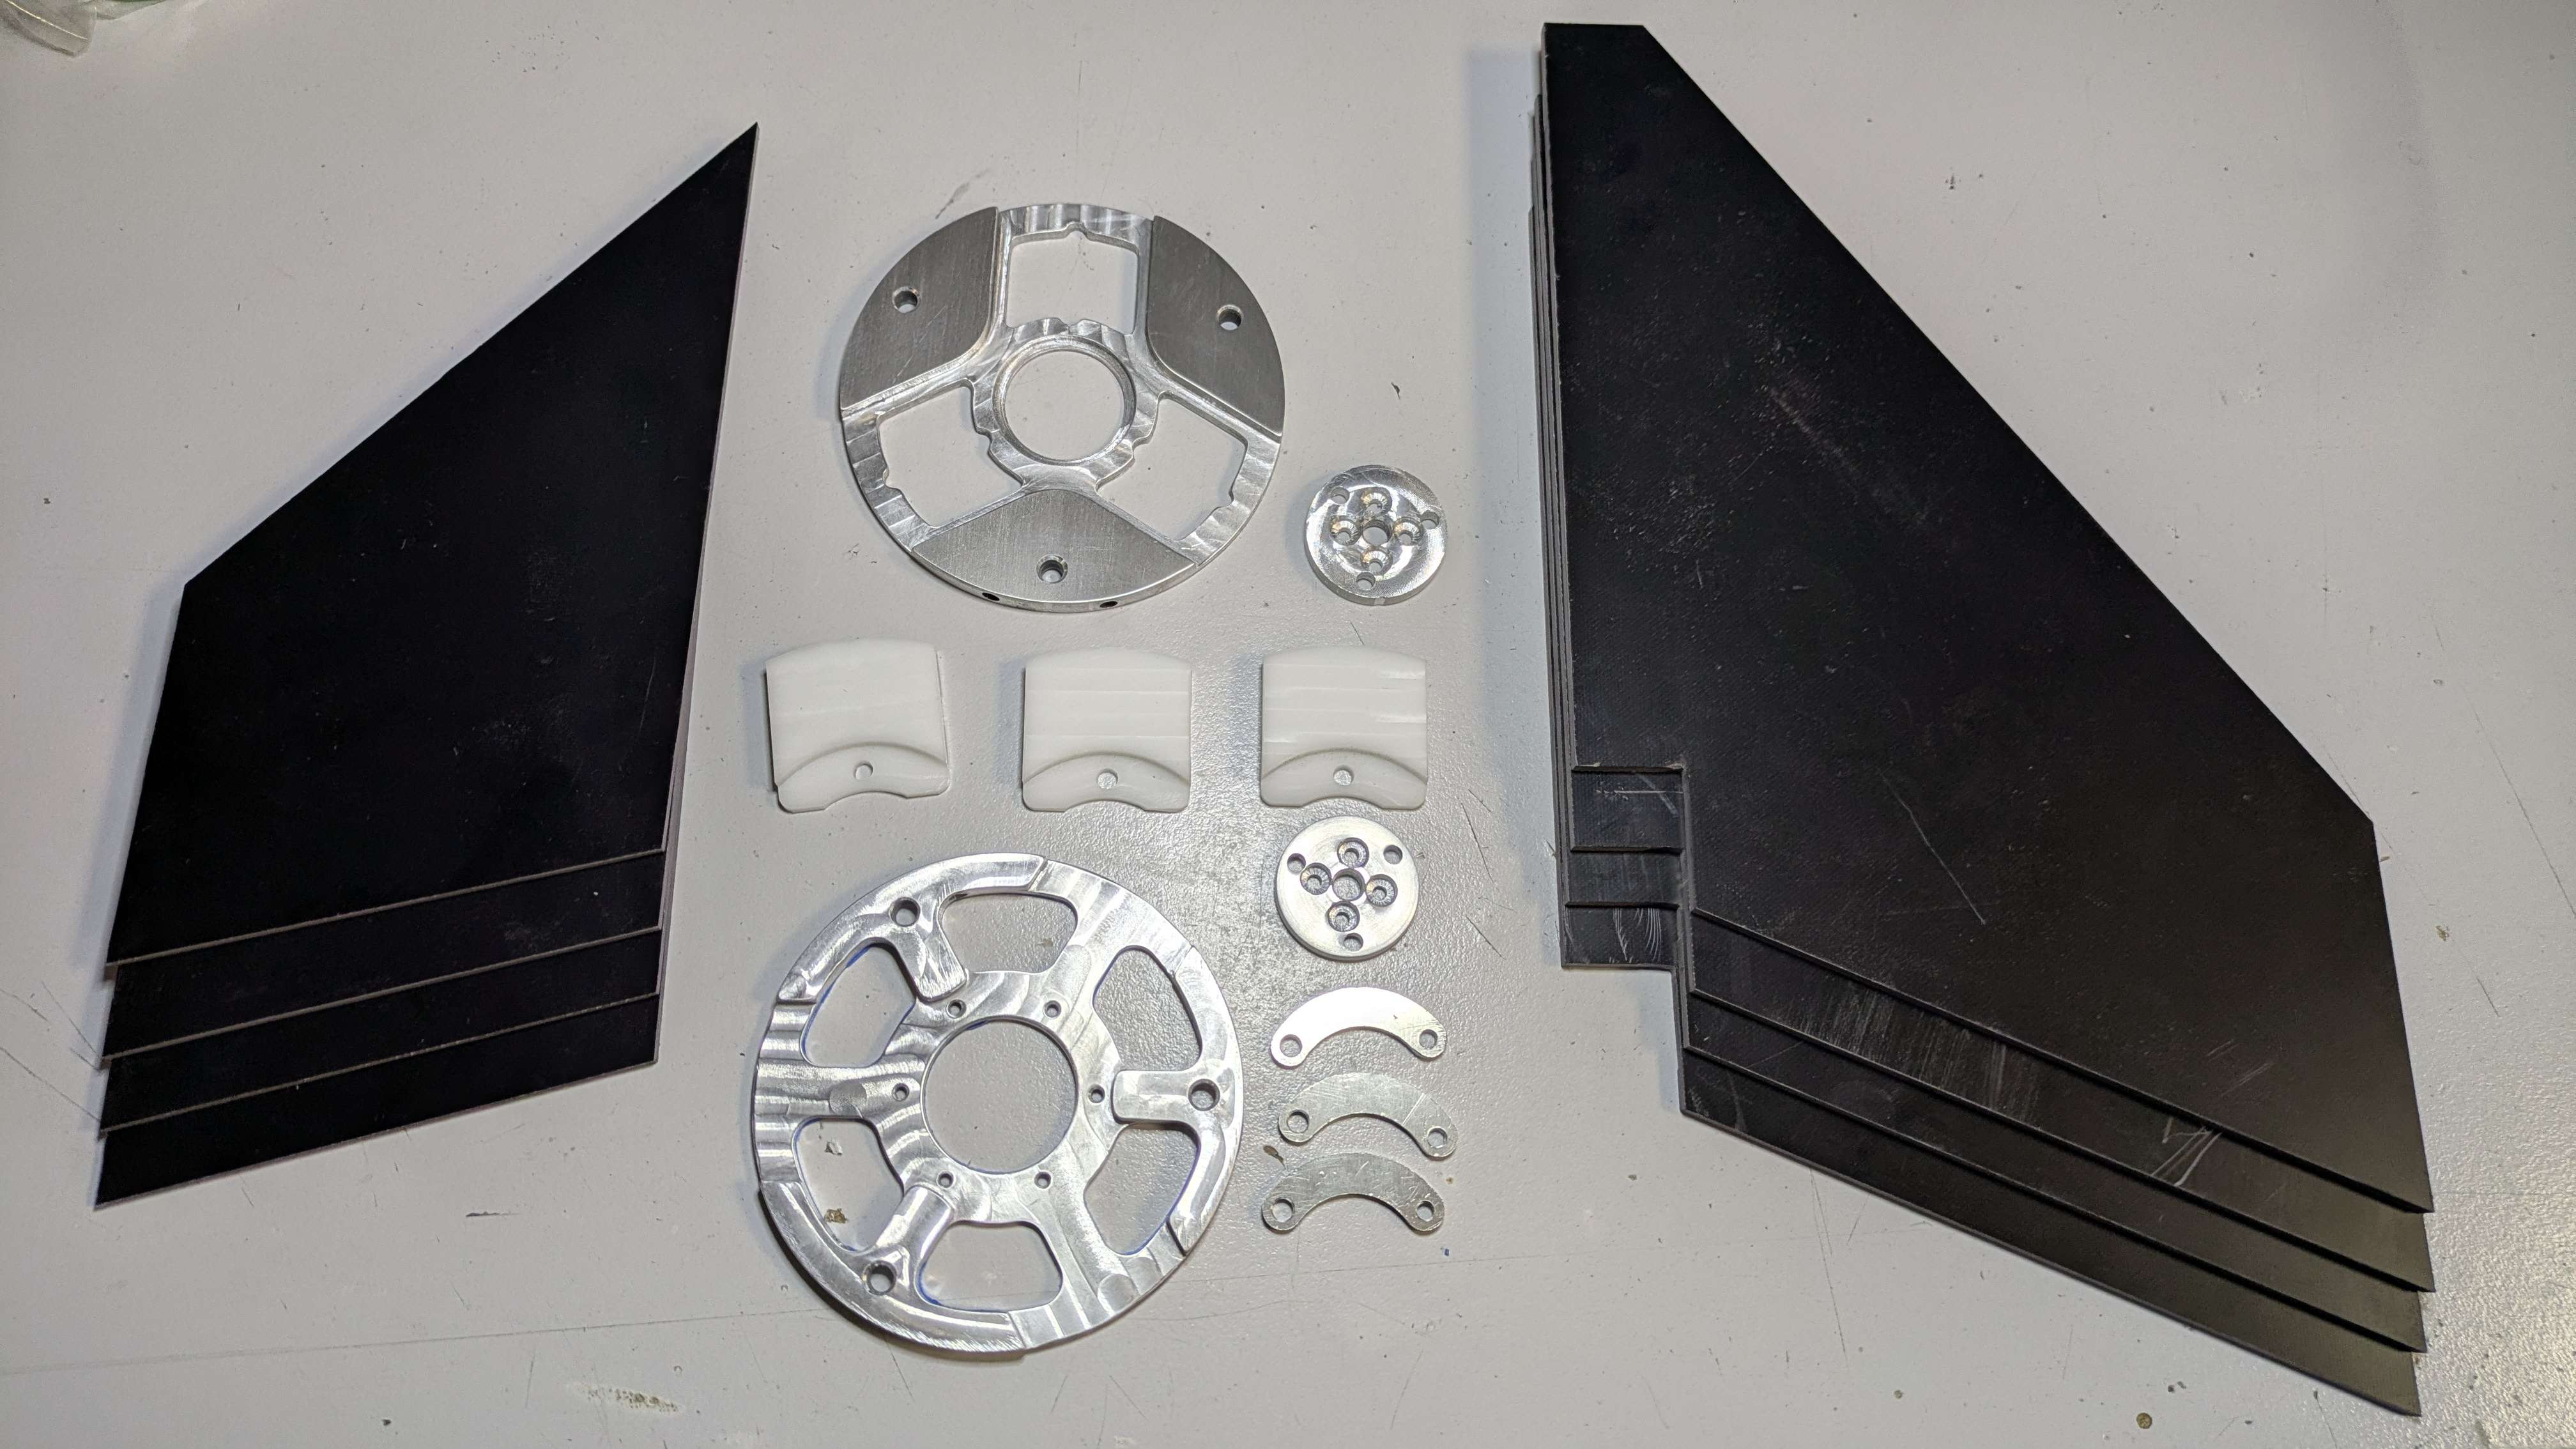
\includegraphics[width=0.7\linewidth]{figures/meca/cnc_pieces_finies.png}
    \caption{Pièces usinées finies : éléments des aérofreins et ailerons.}
    \label{fig:cnc_finies}
\end{figure}




\newpage